\documentclass[10pt,twocolumn]{article}

\usepackage[T1]{fontenc}
\usepackage[utf8]{inputenc}
\usepackage[margin=0.70in,columnsep=0.24in]{geometry}
\usepackage{microtype}
\usepackage{graphicx}
\usepackage{booktabs}
\usepackage{tabularx}
\usepackage{array}
\usepackage{amsmath}
\usepackage{siunitx}
\usepackage{xcolor}
\usepackage[numbers,sort&compress]{natbib}
\usepackage[colorlinks=true,allcolors=blue!55!black]{hyperref}
\usepackage[font=small,labelfont=bf]{caption}
\usepackage{balance}

\newcommand{\code}[1]{\texttt{#1}}
\newcommand{\AUC}{\mathrm{AUROC}}
\newcommand{\dataset}[1]{\textit{#1}}
\renewcommand{\arraystretch}{1.08}
\setlength{\emergencystretch}{1.5em}
% Generated by analysis/dream-consciousness/generate_manuscript_assets.py.
% Do not edit numerical values by hand.
\newcommand{\NremPooledAUC}{0.534}
\newcommand{\NremPooledLow}{0.500}
\newcommand{\NremPooledHigh}{0.569}
\newcommand{\NremSiteMacroAUC}{0.510}
\newcommand{\NremSiteMacroLow}{0.461}
\newcommand{\NremSiteMacroHigh}{0.559}
\newcommand{\NremWithinPairAUC}{0.498}
\newcommand{\NremWithinPairLow}{0.462}
\newcommand{\NremWithinPairHigh}{0.536}
\newcommand{\NremFoldSiteMacroAUC}{0.524}
\newcommand{\NremFoldSiteMacroLow}{0.473}
\newcommand{\NremFoldSiteMacroHigh}{0.577}
\newcommand{\NremFoldWithinPairAUC}{0.509}
\newcommand{\NremFoldWithinPairLow}{0.471}
\newcommand{\NremFoldWithinPairHigh}{0.551}
\newcommand{\NremFoldDelta}{0.009}
\newcommand{\NremFoldDeltaLow}{-0.029}
\newcommand{\NremFoldDeltaHigh}{0.051}
\newcommand{\NremWithinPairFraction}{30.6\%}
\newcommand{\NremCrossPairFraction}{69.4\%}
\newcommand{\NremCrossConcordance}{0.550}
\newcommand{\NremRandomAUC}{0.569}
\newcommand{\NremLegacyParticipantAUC}{0.550}
\newcommand{\NremLaboratoryAUC}{0.493}
\newcommand{\NremSiteOnlyPooledAUC}{0.564}
\newcommand{\NremSiteOnlyPooledLow}{0.511}
\newcommand{\NremSiteOnlyPooledHigh}{0.616}
\newcommand{\RemPooledAUC}{0.629}
\newcommand{\RemPooledLow}{0.567}
\newcommand{\RemPooledHigh}{0.701}
\newcommand{\RemSiteMacroAUC}{0.498}
\newcommand{\RemSiteMacroLow}{0.439}
\newcommand{\RemSiteMacroHigh}{0.595}
\newcommand{\RemWithinPairAUC}{0.498}
\newcommand{\RemWithinPairLow}{0.440}
\newcommand{\RemWithinPairHigh}{0.576}
\newcommand{\RemFoldSiteMacroAUC}{0.555}
\newcommand{\RemFoldSiteMacroLow}{0.502}
\newcommand{\RemFoldSiteMacroHigh}{0.644}
\newcommand{\RemFoldWithinPairAUC}{0.552}
\newcommand{\RemFoldWithinPairLow}{0.501}
\newcommand{\RemFoldWithinPairHigh}{0.643}
\newcommand{\RemFoldDelta}{0.052}
\newcommand{\RemFoldDeltaLow}{0.001}
\newcommand{\RemFoldDeltaHigh}{0.143}
\newcommand{\RemWithinPairFraction}{30.0\%}
\newcommand{\RemCrossPairFraction}{70.0\%}
\newcommand{\RemCrossConcordance}{0.685}
\newcommand{\RemRandomAUC}{0.636}
\newcommand{\RemLegacyParticipantAUC}{0.663}
\newcommand{\RemLaboratoryAUC}{0.470}
\newcommand{\RemSiteOnlyPooledAUC}{0.687}
\newcommand{\RemSiteOnlyPooledLow}{0.611}
\newcommand{\RemSiteOnlyPooledHigh}{0.767}
\newcommand{\RemNoTurkuPooledAUC}{0.560}
\newcommand{\RemNoTurkuPooledLow}{0.495}
\newcommand{\RemNoTurkuPooledHigh}{0.638}
\newcommand{\RemNoTurkuWithinPairAUC}{0.514}
\newcommand{\RemNoTurkuWithinPairLow}{0.457}
\newcommand{\RemNoTurkuWithinPairHigh}{0.595}
\newcommand{\RemNoTurkuFoldWithinPairAUC}{0.563}
\newcommand{\RemNoTurkuFoldWithinPairLow}{0.510}
\newcommand{\RemNoTurkuFoldWithinPairHigh}{0.659}
\newcommand{\NremIdentityMin}{0.770}
\newcommand{\NremIdentityMax}{0.940}
\newcommand{\RemIdentityMin}{0.627}
\newcommand{\RemIdentityMax}{0.953}
\newcommand{\PublishedIdentityMin}{0.808}
\newcommand{\PublishedIdentityMax}{0.953}
\newcommand{\RemRawIrrevLaboratoryAUC}{0.604}
\newcommand{\RemSurrogateIrrevLaboratoryAUC}{0.490}
\newcommand{\NremLaboratoryParticipantEqualAUC}{0.484}
\newcommand{\RemLaboratoryParticipantEqualAUC}{0.454}

\hypersetup{
  pdftitle={Cross-Laboratory Validation of EEG Classification of Reported Dream Experience},
  pdfauthor={Javier Emilio Bazan Sanchez}
}

\title{Cross-Laboratory Validation of EEG Classification\\
of Reported Dream Experience}
\author{Javier Emilio Baz\'an S\'anchez \quad
\normalsize\href{mailto:bazan@ciencias.unam.mx}{\texttt{bazan@ciencias.unam.mx}}}
\date{2 August 2026}

\begin{document}
\maketitle

\begin{abstract}
Electroencephalographic classifiers of reported dream experience may exploit
laboratory structure even when participants are held out. We audited the
released DREAM Figure~5 workflow and analyzed 1,065 strict binary reports from
five collections (730 NREM; 335 REM). A close adaptation approximately
recovered record-wise discrimination (NREM spectral power,
$\AUC=\NremRandomAUC$; REM filtered Catch22, $\AUC=\RemRandomAUC$). With
participant-held-out predictions pooled across laboratories, AUROC was
\NremPooledAUC\ [\NremPooledLow, \NremPooledHigh] and
\RemPooledAUC\ [\RemPooledLow, \RemPooledHigh], respectively. Restricting
concordant pairs to the same laboratory reduced both primary estimates to
approximately chance (\NremWithinPairAUC\ [\NremWithinPairLow,
\NremWithinPairHigh] and \RemWithinPairAUC\ [\RemWithinPairLow,
\RemWithinPairHigh]). A classifier using only training-fold laboratory
prevalence attained pooled AUROCs of \NremSiteOnlyPooledAUC\ and
\RemSiteOnlyPooledAUC. Cross-laboratory comparisons constituted
\NremCrossPairFraction\ of NREM and \RemCrossPairFraction\ of REM pooled
positive--negative pairs. When a whole laboratory was held out, primary
performance was \NremLaboratoryAUC\ and \RemLaboratoryAUC. Conversely,
laboratory identity was readily decoded from published feature families
($\AUC=\PublishedIdentityMin$--$\PublishedIdentityMax$). Within-laboratory REM
performance was estimator- and collection-dependent, including a
fold-conditioned sensitivity of \RemFoldWithinPairAUC\ and
\RemNoTurkuFoldWithinPairAUC\ after excluding the severely imbalanced Turku
collection. Across the tested DREAM collections, the released workflow
supports pooled discriminability but does not establish a common,
transportable EEG marker of reported dream experience.
\end{abstract}

\section{Introduction}

Dream reports pose a distinctive measurement problem: the target experience
is private, and its label is observed only after awakening. The DREAM database
harmonized multiple EEG and mentation collections and reported that spectral
power and Catch22 features discriminated ``Experience'' from ``No experience''
under pooled random splitting \citep{wong2025dream,lubba2019catch22}. This is an
important benchmark, but a pooled multicenter AUROC is not a single-domain
quantity.

Participant separation and laboratory separation answer different scientific
questions. Participant-held-out validation tests whether a rule generalizes
to new people while acquisition domains remain represented on both sides of
the split. Laboratory-held-out validation tests transport to a new acquisition
and reporting domain. Between those levels lies a diagnostic estimand:
site-conditioned AUROC, which asks whether held-out participants with and
without reported experience are ranked correctly when both records came from
the same laboratory. If label prevalence and score location differ by site,
pooled AUROC may be high even when within-site ranking is absent. This is a
form of domain confounding distinct from direct participant leakage
\citep{varoquaux2018crossvalidation,kapoor2023leakage}.

Prior dream-decoding studies include blinded spectral-power tests and
single-collection classifiers \citep{wong2020catcher,moctezuma2025unlocking},
but our focused search did not identify an earlier laboratory-held-out
evaluation of the exact DREAM Figure~5 workflow. We therefore performed a
reproducibility and falsification analysis with five levels: record-wise
discrimination, participant-held-out pooled discrimination, participant-held-
out site-conditioned discrimination, laboratory-held-out transport, and
laboratory-identity and prevalence-only controls. We also retained two
mechanistically motivated extensions---Riemannian covariance and temporal
irreversibility---with alignment and spectral-surrogate controls
\citep{barachant2012riemann,zanini2018transfer,delafuente2023time}.

\section{Materials and Methods}

\subsection{Source audit and analytic sample}

We retrieved the versioned public collections enumerated by the deposited
Figure~5 code and verified archives against publisher-provided sizes and MD5
digests. DREAM code 2 (Experience) was mapped to 1 and code 0 (No experience)
to 0. Experience without recall, ambiguous or unknown labels, and wake
observations were excluded. Subject identifiers were scoped jointly by source
collection and original identifier. Three Young Adults EDFs fail CRC despite
the archive matching its published MD5, and one Turku EDF is absent from its
archive; these records were excluded.

The paper describes six collections across its broader EEG analyses, whereas
the Figure~5 classifier lists five. We did not add Oudiette N1Data post hoc:
its sleeping subset contains only one strict No-experience report, and its
Fp1/C3/O1 montage does not match the classifier's F4/C4/O2 montage. The final
code-path sample contained 1,065 reports from 166 unique participants. Because
prevalence is part of the confounding question, Table~\ref{tab:composition}
reports counts separately by sleep stage and collection.

\begin{table*}[t]
\centering
\caption{Stage-specific analytic composition. Experience prevalence is
computed after all exclusions. Participants contributing both stages are
counted in each stage. $^{*}$Fewer than five No-experience records; within-site
AUROC is correspondingly fragile.}
\label{tab:composition}
\small
\begin{tabular}{llrrrrr}
\toprule
Stage & Collection & Participants & Records & Experience & No experience & Experience (\%) \\
\midrule
% Generated stage-specific composition rows.
NREM & Young Adults & 32 & 32 & 18 & 14 & 56.2\% \\
NREM & Multiple Awakenings & 19 & 281 & 189 & 92 & 67.3\% \\
NREM & Siclari & 39 & 231 & 124 & 107 & 53.7\% \\
NREM & Zhang & 27 & 186 & 139 & 47 & 74.7\% \\
REM & Young Adults & 30 & 30 & 20 & 10 & 66.7\% \\
REM & Multiple Awakenings & 19 & 154 & 125 & 29 & 81.2\% \\
REM & Zhang & 20 & 26 & 17 & 9 & 65.4\% \\
REM & Turku$^{*}$ & 18 & 125 & 122 & 3 & 97.6\% \\
\bottomrule

\end{tabular}
\end{table*}

\subsection{Reproduction boundary and features}

Literal execution of the deposit is blocked by three documented gaps. It
imports a missing \code{feat\_ext\_funcs} module; it specifies a semicolon
delimiter for a public comma-delimited records file; and it expects Siclari
\code{formatted\_*.edf} files and F4-M1/C4-M1/O2-M1 channels absent from all
public versions inspected. We computed filtered Catch22 directly with
\code{pycatch22} and reconstructed Siclari F4/C4/O2-M1 from the nearest
HydroCel-256 sensors. These adaptations permit conceptual, not exact numerical,
reproduction.

We analyzed the final 30~s before each report and resampled signals to 128~Hz
for time-series features. Published families comprised normalized multitaper
power in six bands across three channels, broadband Catch22, and Catch22 after
six band-pass filters. Covariance matrices were trace-normalized, shrunk by one
percent, and represented in a log-Euclidean tangent space. A label-free
transductive alignment subtracted each laboratory--stage log-Euclidean mean.
Temporal irreversibility used ordinal-pattern Jensen--Shannon divergence and a
cubic time-asymmetry statistic at four lags. Twenty-four deterministic phase-
randomized surrogates per channel provided a spectrum-preserving control.

\subsection{Models and validation estimands}

Binary models used the released XGBoost settings: learning rate 0.1, depth 3,
subsampling 0.8, feature subsampling 0.8, and the workflow's implicit default
of ten boosting rounds \citep{chen2016xgboost}. No feature-family-specific
optimization was performed. Random-record and participant-held-out analyses
used five folds and 20 deterministic shuffled repetitions. Participant folds
were generated by stratified group cross-validation, with no participant in
both train and test partitions.

For each repetition, \emph{pooled participant-held-out AUROC} compared every
out-of-fold positive with every out-of-fold negative, regardless of source.
\emph{Site-conditioned AUROC} retained only positive--negative pairs from the
same laboratory. We report both a macro average giving each eligible
laboratory equal weight and a pair-weighted value giving each within-site pair
equal weight. \emph{Participant-equal} estimates assigned each participant a
total weight of one before forming pairs. \emph{Laboratory-held-out AUROC}
trained on all other collections and evaluated the untouched target; its
summary is the unweighted mean across four eligible target laboratories per
stage.

A site-only baseline assigned each test record the experience prevalence of
its laboratory estimated from the corresponding training fold; no test labels
were used. Because training prevalence varies inversely with held-out fold
composition, direct pooling across mutually exclusive test folds can induce an
artificial within-site ordering even for this constant-within-fold baseline.
After observing this evaluation artifact, we added a transparently labeled
estimator clarification: fold-conditioned site AUROC, which restricts pairs to
the same laboratory \emph{and} test fold. The site-only baseline is exactly
0.5 under this estimand. This sensitivity was not used to select models.

AUROC was decomposed exactly into concordant within-site and cross-site pair
contributions. Uncertainty used 2,000 participant-cluster bootstrap samples,
resampling participants independently within each laboratory while retaining
all their observations. The primary families were fixed before analysis as
NREM spectral power and REM filtered Catch22. Frozen sensitivities included
participant-equal weighting, site macro weighting, REM with Turku excluded,
and the full pre-existing feature set.

\section{Results}

\subsection{Approximate benchmark recovery}

The adapted workflow recovered the scale and direction of the published
benchmark. NREM spectral power reached record-wise $\AUC=\NremRandomAUC$
(DREAM: 0.586); REM filtered Catch22 reached $\AUC=\RemRandomAUC$ (DREAM:
0.700). The discrepancy is consistent with the missing feature module and
unavailable Siclari preprocessing, so these values are treated as an
approximate code-path reproduction.

Earlier fold-mean participant-held-out summaries were
$\AUC=\NremLegacyParticipantAUC$ and \RemLegacyParticipantAUC. Reconstructing
record-level out-of-fold probabilities allowed estimands to be evaluated on a
common prediction set. Pooled participant-held-out AUROC was
\NremPooledAUC\ [\NremPooledLow, \NremPooledHigh] for NREM spectral power and
\RemPooledAUC\ [\RemPooledLow, \RemPooledHigh] for REM filtered Catch22. The
change from the earlier summaries reflects fold-mean versus pooled-pair
weighting, not retraining on different records.

\subsection{Pooled and site-conditioned performance diverge}

Restricting comparisons to records from the same laboratory reduced the
primary pair-weighted AUROCs to \NremWithinPairAUC\ [\NremWithinPairLow,
\NremWithinPairHigh] for NREM and \RemWithinPairAUC\ [\RemWithinPairLow,
\RemWithinPairHigh] for REM. Equal-laboratory macro estimates were
\NremSiteMacroAUC\ [\NremSiteMacroLow, \NremSiteMacroHigh] and
\RemSiteMacroAUC\ [\RemSiteMacroLow, \RemSiteMacroHigh]. Thus, the primary
pooled estimates did not describe a common within-laboratory ordering.

Results were heterogeneous rather than uniformly null. NREM spectral power
was above chance in Zhang but near or below chance in the other collections;
REM filtered Catch22 was below chance in the extremely imbalanced Turku
collection and imprecisely above chance in Zhang (Supplementary
Table~\ref{tab:sites}). The fold-conditioned pair-weighted sensitivity was
\NremFoldWithinPairAUC\ [\NremFoldWithinPairLow, \NremFoldWithinPairHigh] for
NREM and \RemFoldWithinPairAUC\ [\RemFoldWithinPairLow,
\RemFoldWithinPairHigh] for REM. The corresponding differences from the
0.5 site-only baseline were \NremFoldDelta\ [\NremFoldDeltaLow,
\NremFoldDeltaHigh] and \RemFoldDelta\ [\RemFoldDeltaLow,
\RemFoldDeltaHigh]. Excluding Turku changed the REM fold-conditioned estimate
to \RemNoTurkuFoldWithinPairAUC\ [\RemNoTurkuFoldWithinPairLow,
\RemNoTurkuFoldWithinPairHigh], confirming sensitivity to collection
composition rather than a stable common effect.

\subsection{Site-only prediction and pair decomposition}

Using no EEG features, training-fold site prevalence produced pooled AUROCs of
\NremSiteOnlyPooledAUC\ [\NremSiteOnlyPooledLow, \NremSiteOnlyPooledHigh] in
NREM and \RemSiteOnlyPooledAUC\ [\RemSiteOnlyPooledLow,
\RemSiteOnlyPooledHigh] in REM. This does not imply that the EEG model is
equivalent to the baseline; it shows that laboratory membership alone carries
substantial pooled ranking information.

The pair decomposition identifies where the primary pooled AUROC originates
(Figure~\ref{fig:pairs}). Within-site pairs comprised only
\NremWithinPairFraction\ of NREM and \RemWithinPairFraction\ of REM pairs.
Their concordances were \NremWithinPairAUC\ and \RemWithinPairAUC, whereas
cross-site concordances were \NremCrossConcordance\ and
\RemCrossConcordance. The weighted within- and cross-site contributions
reconstruct the pooled AUROC to machine precision. Directional off-diagonal
cells also reveal that a score's ranking can reverse with the source pairing.

\begin{figure*}[t]
\centering
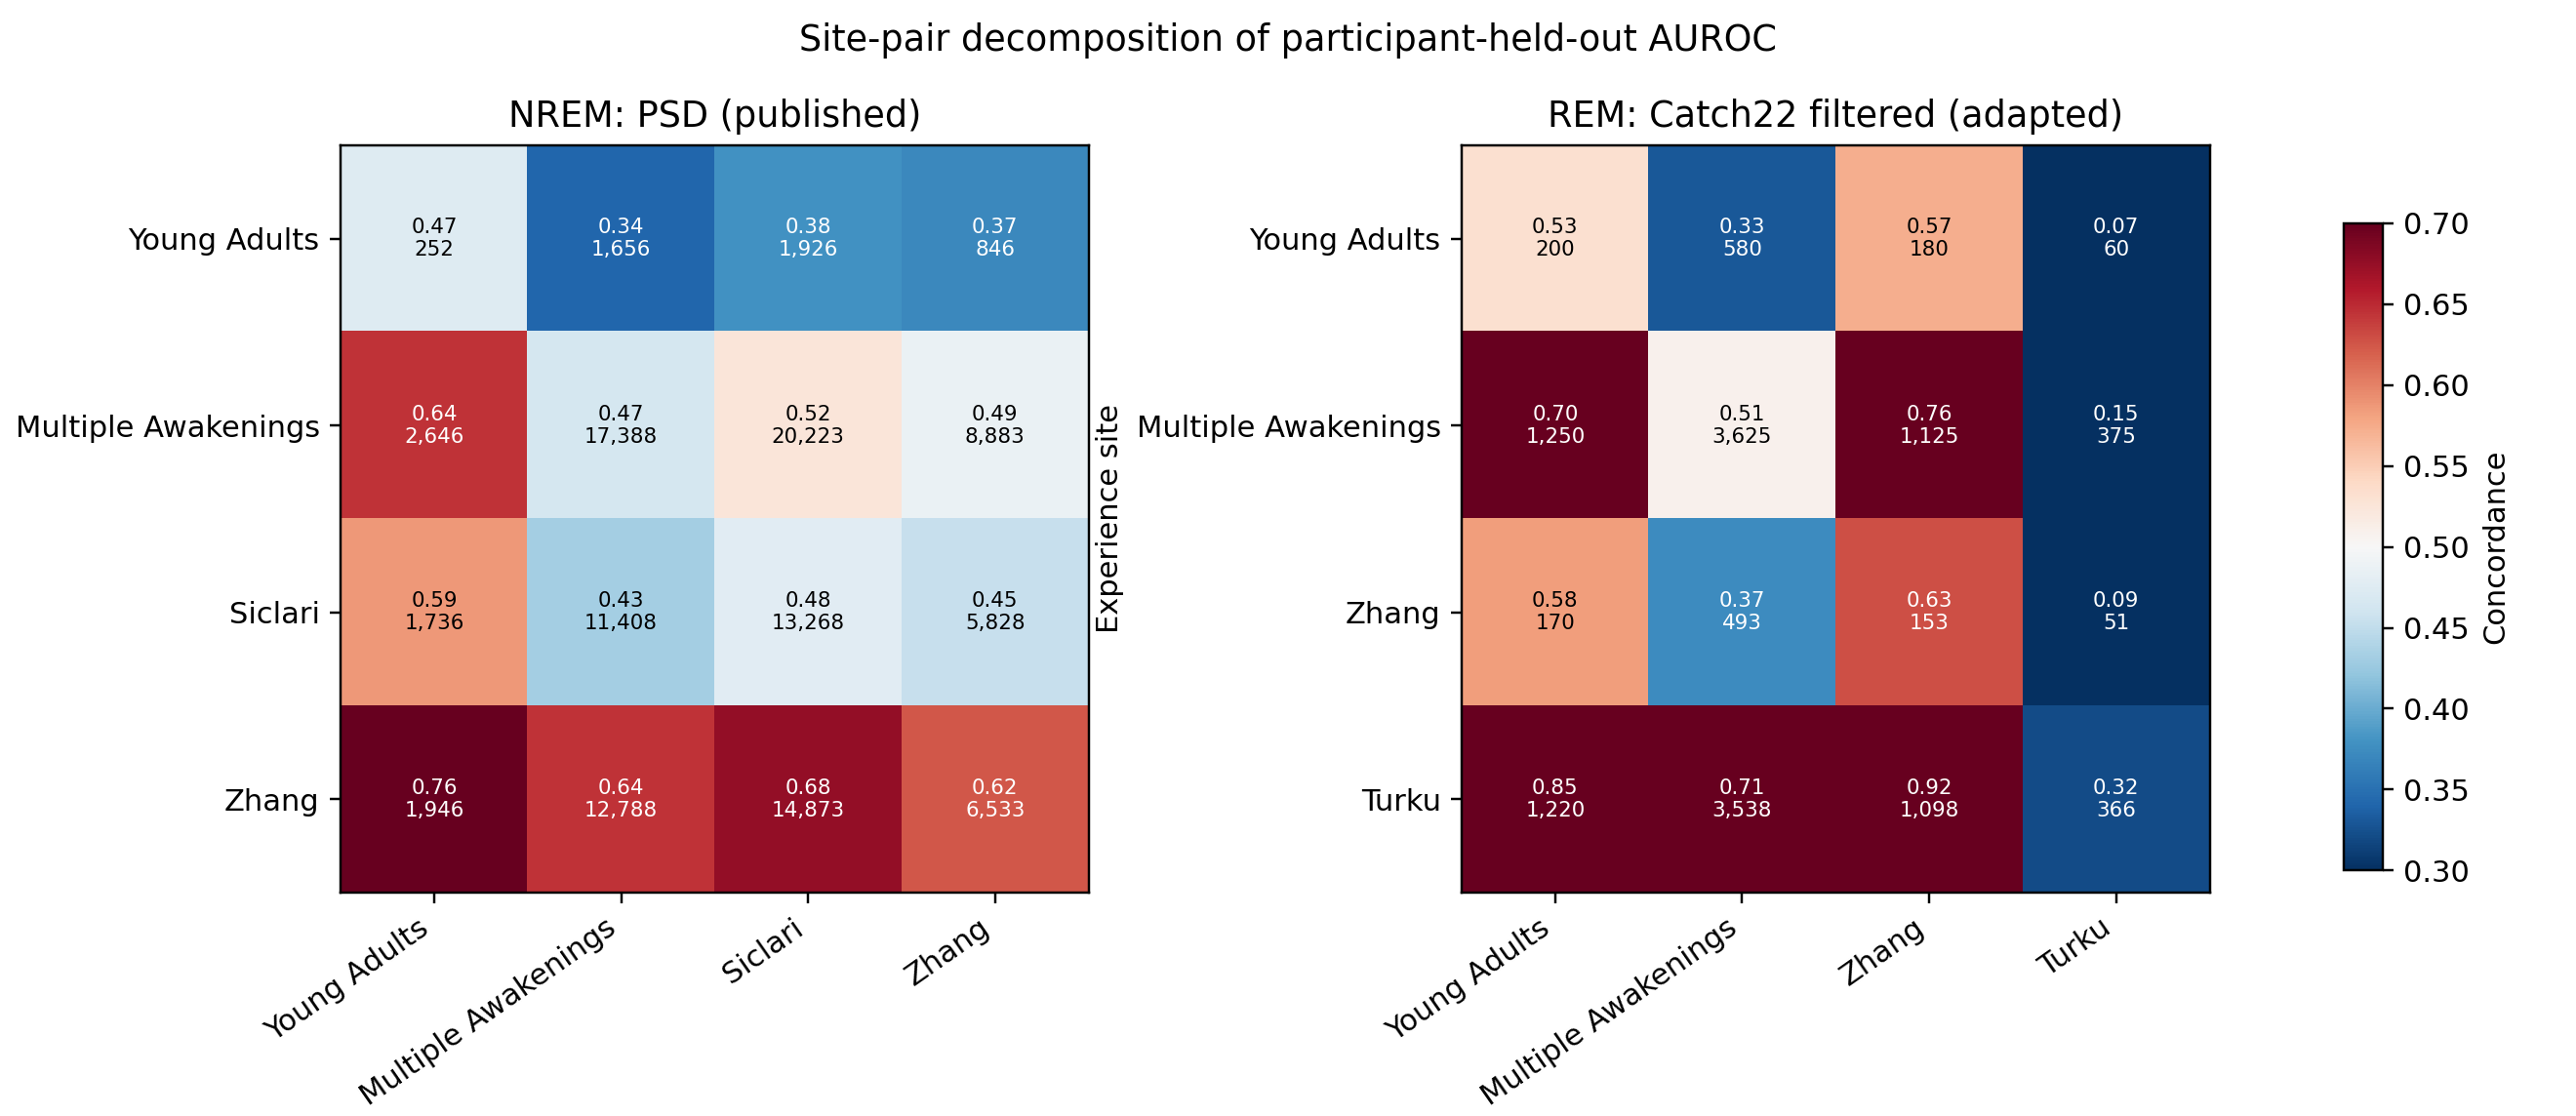
\includegraphics[width=0.98\textwidth]{figures/site-pair-heatmaps.png}
\caption{Exact site-pair decomposition of participant-held-out pooled AUROC
for the two primary models. Rows identify the source of Experience records and
columns the source of No-experience records. Each cell reports concordance
(top) and the number of positive--negative pairs (bottom), averaged over the
fixed repeated folds where appropriate. Diagonal cells are within-site;
off-diagonal cells are cross-site.}
\label{fig:pairs}
\end{figure*}

\subsection{Performance does not transport to every laboratory}

With an entire laboratory held out, the primary macro AUROCs were
\NremLaboratoryAUC\ for NREM spectral power and \RemLaboratoryAUC\ for REM
filtered Catch22; participant-equal summaries were
\NremLaboratoryParticipantEqualAUC\ and
\RemLaboratoryParticipantEqualAUC. Target estimates varied widely
(Figure~\ref{fig:targets}), and no primary model had a favorable
participant-cluster interval excluding 0.5 in every target. Turku contains
only three No-experience records, making its REM interval and any aggregate
that includes it especially unstable.

\begin{figure*}[t]
\centering
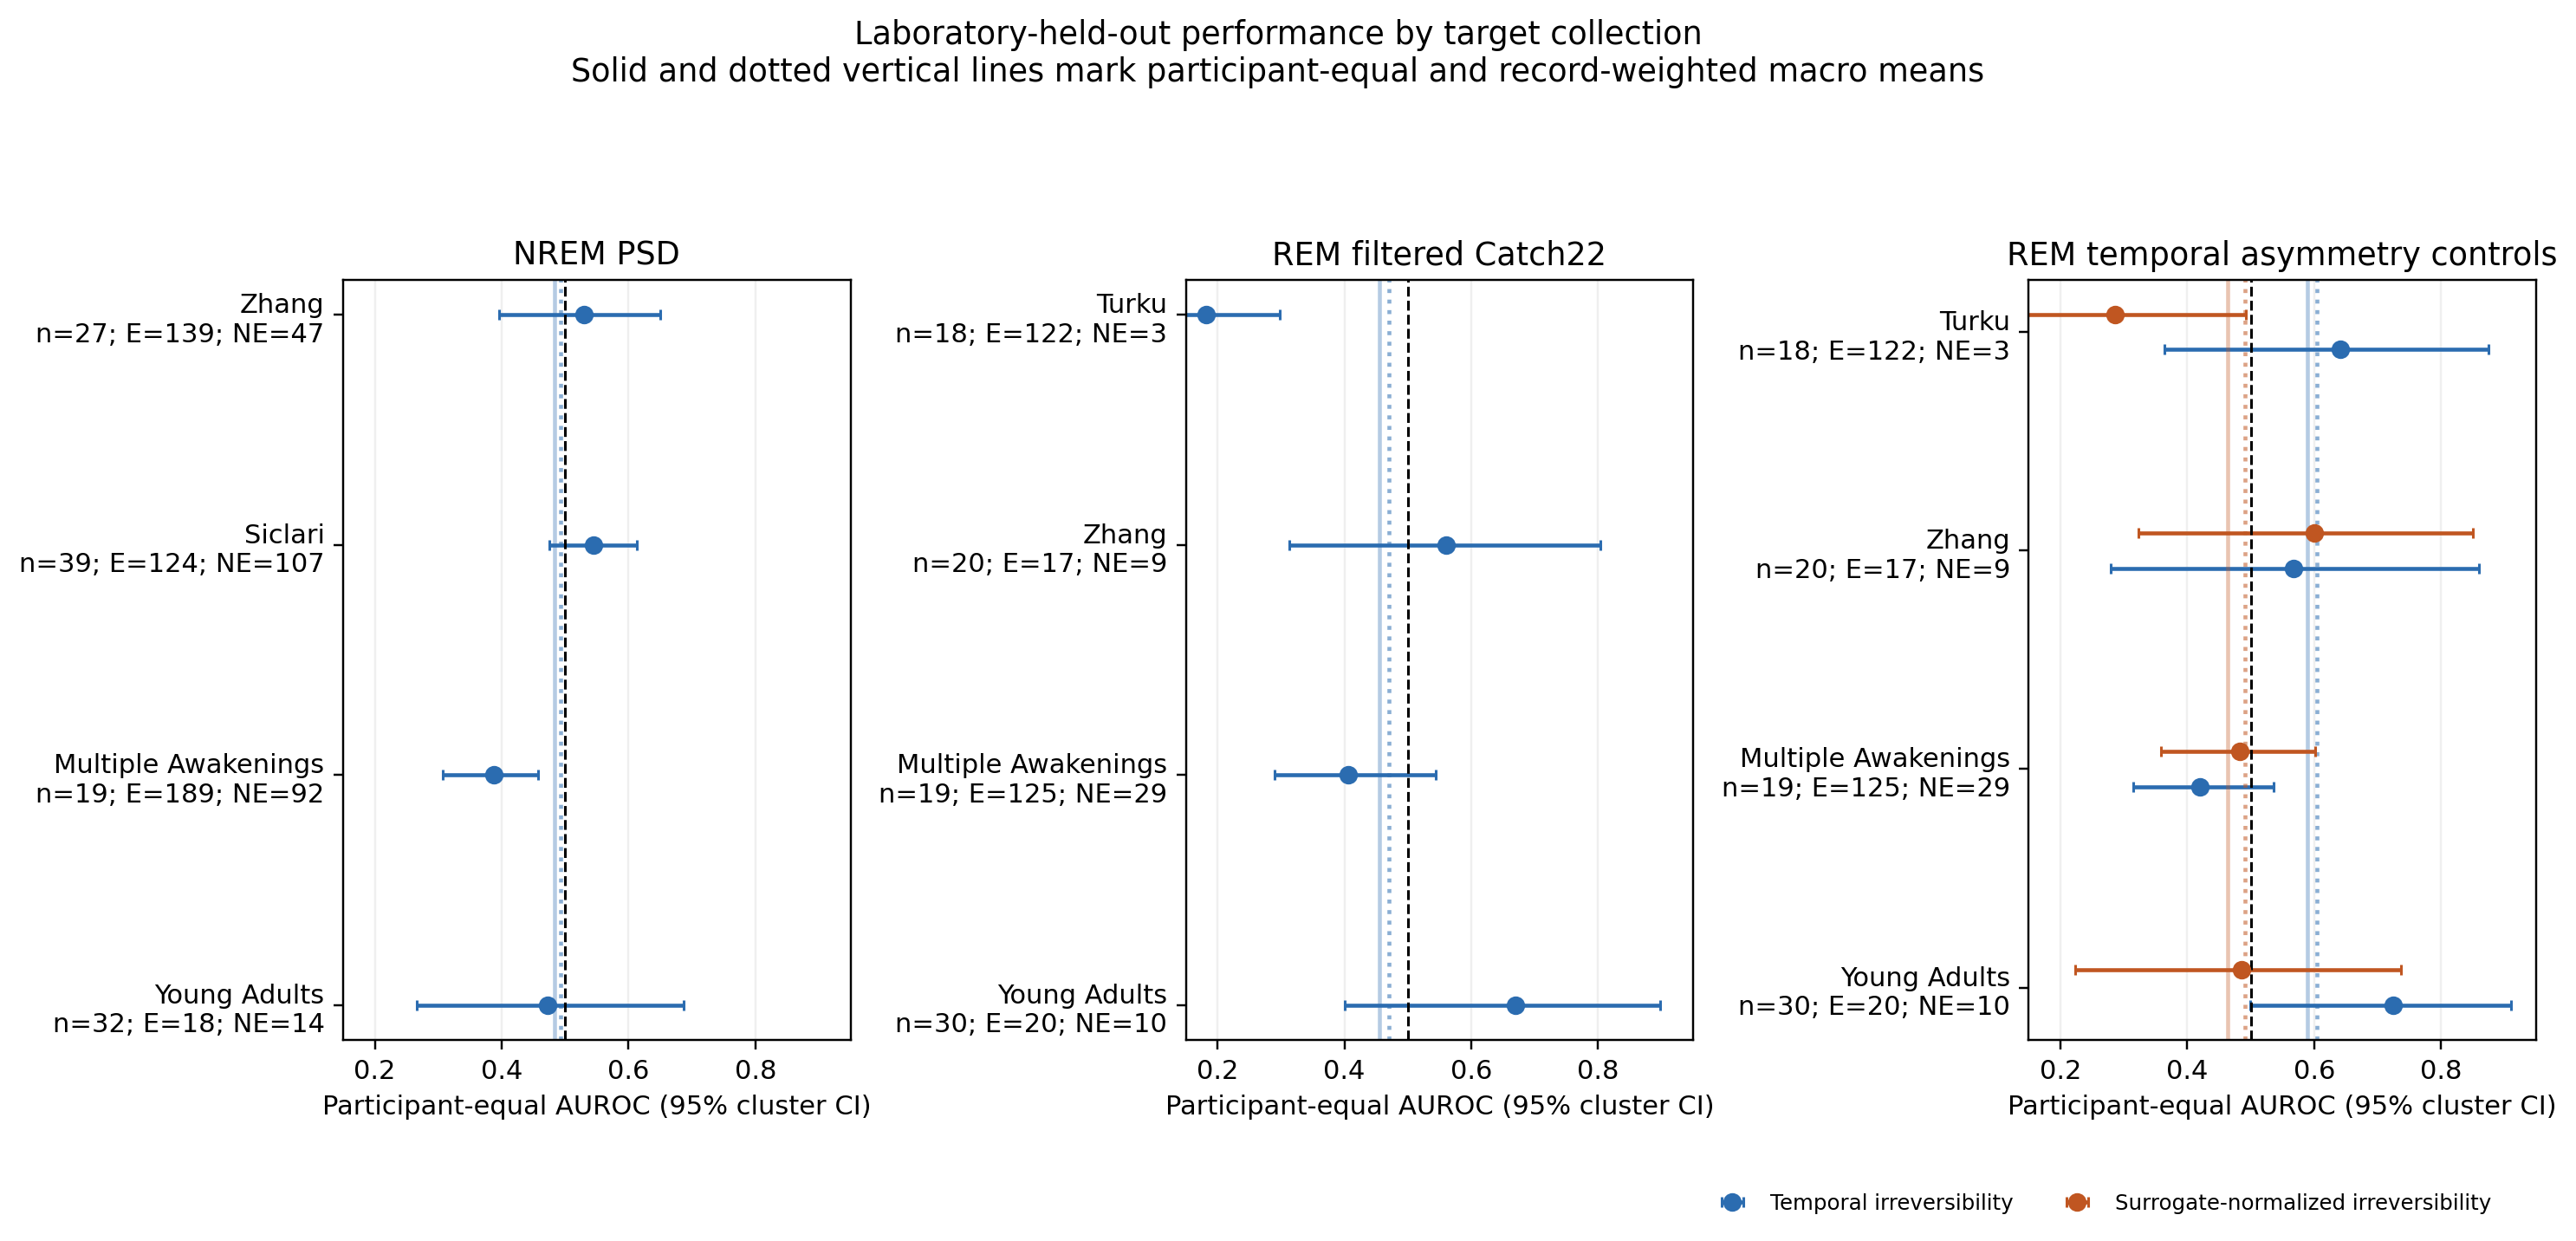
\includegraphics[width=0.99\textwidth]{figures/target-laboratory-forest.png}
\caption{Laboratory-held-out participant-equal AUROC with 95\% participant-
cluster bootstrap intervals. The first two panels show the fixed primary
models. The third shows raw temporal irreversibility (blue) and its phase-
surrogate-normalized control (orange). Solid and dotted vertical lines are
participant-equal and record-weighted macro means. E and NE denote Experience
and No-experience records.}
\label{fig:targets}
\end{figure*}

\subsection{Laboratory identity and mechanistic controls}

Laboratory identity remained strongly decodable under participant-held-out
evaluation. Across PSD, broadband Catch22, and filtered Catch22, macro AUROC
ranged from \PublishedIdentityMin\ to \PublishedIdentityMax. This establishes
large residual domain information but does not prove that every experience
prediction is artifactual.

Neither advanced representation supplied a robust rescue. Riemannian
covariance and label-free log-Euclidean alignment remained heterogeneous
across laboratories (Supplementary Table~\ref{tab:secondary}). Raw temporal
irreversibility was the strongest exploratory REM family under laboratory
shift ($\AUC=\RemRawIrrevLaboratoryAUC$), but fell to
$\AUC=\RemSurrogateIrrevLaboratoryAUC$ after normalization against
phase-randomized surrogates. Because those surrogates preserve each channel's
spectrum while disrupting nonlinear temporal ordering, this reduction does
not support a domain-invariant arrow-of-time interpretation for the tested
statistics.

\section{Discussion}

The principal result is a separation of estimands. The released workflow
approximately reproduces pooled record-wise discriminability. Some pooled
participant-held-out discrimination remains when people are separated. Yet
the two primary models are approximately chance when positive--negative pairs
are restricted to the same laboratory, and their decision rules do not
transport consistently to an unseen laboratory. Participant-held-out
validation therefore preserved an apparently successful multicenter benchmark
while leaving laboratory-level structure shared across training and test data.

The site-only baseline and pair decomposition clarify, but do not fully
causally explain, that divergence. About seven in ten pooled pairs were
cross-laboratory comparisons. Such comparisons can reward stable differences
in score location that covary with laboratory prevalence, acquisition, or
reporting protocol without requiring within-laboratory experience ranking.
Conversely, the fold-conditioned REM sensitivity was modestly above 0.5 and
increased after excluding Turku. The appropriate interpretation is therefore
heterogeneity: the pooled benchmark combines collection-specific effects, and
a reproducible within-domain signal may exist in some settings, but a common
transportable marker has not been established.

The mathematical extensions are informative chiefly as falsification tests.
Riemannian geometry is principled for covariance-domain shift, but only three
common channels with heterogeneous references were available. Log-Euclidean
centering removes a domain mean, not arbitrary changes in covariance or label
semantics. Temporal irreversibility has a plausible link to conscious dynamics,
yet the phase-surrogate control shows why mechanistic null models are necessary
before attributing performance to nonlinear temporal direction.

These findings do not show that EEG lacks correlates of dreaming. The labels
themselves are imperfect proxies: ``No experience'' may combine absent
experience, failed encoding, forgetting, and protocol-specific categorization.
Failure across collections can therefore reflect genuine construct
heterogeneity as well as instrumentation and preprocessing shift. A stronger
future design would prospectively harmonize channels, reference, awakenings,
question wording, and class balance, then reserve laboratories for external
validation from the outset.

\subsection{Limitations}

This reanalysis was exploratory rather than preregistered; the targeted
diagnostic protocol was frozen only before the new site-conditioned runs. The
missing feature module and reconstructed Siclari channels preclude exact
numerical reproduction. Each stage has only four eligible target laboratories,
and Turku is severely imbalanced. Analyses used three common channels and the
final 30~s only. Participant-cluster bootstrap intervals do not capture
uncertainty over a wider population of laboratories. Log-Euclidean alignment
is transductive because it uses the unlabeled target batch. Finally, the
novelty search was focused, not a registered systematic review; to our
knowledge, we did not identify an earlier laboratory-held-out evaluation of
this exact workflow.

\section{Conclusion}

Across the tested DREAM collections, the released Figure~5 workflow supports
pooled discriminability but does not yet establish a transportable EEG marker
of reported dream experience. Participant separation, site-conditioned
ranking, site-prevalence baselines, dataset-identity controls, and unseen-
laboratory validation should be reported as distinct tests in multicenter
dream decoding.

\section*{Data and code availability}

The public reproducibility repository at
\href{https://github.com/asim-v/dream-decoder-generalization-paper}{github.com/asim-v/dream-decoder-generalization-paper}
contains the frozen feature matrices, deterministic folds, complete out-of-fold
probabilities, machine-readable results, tests, table and figure generators,
environment lockfile, LaTeX source, and compiled PDF. One top-level command
recreates the diagnostics and manuscript assets from the redistributed derived
features. Raw EEG is not redistributed; the README provides persistent source
identifiers, sizes, hashes, and acquisition instructions. Exact reproduction
of the upstream Figure~5 feature matrix remains blocked by the unreleased
\code{feat\_ext\_funcs} module and preformatted Siclari files expected by the
deposit.

\section*{Ethics statement}

This study reanalyzed de-identified public data and did not recruit
participants or modify source records. Ethical approvals and consent
procedures are described in the originating studies and DREAM records.

\section*{Competing interests}

The author declares no competing interests.

\clearpage
\appendix
\onecolumn
\section{Supplementary results}

\begin{table}[h]
\centering
\caption{Primary participant-held-out within-site AUROC by collection. Values
use record-weighted pairs; intervals resample participants within collection.
E and NE are the two strict report classes.}
\label{tab:sites}
\small
\begin{tabular}{llrrrr}
\toprule
Stage & Collection & Participants & E & NE & AUROC [95\% CI] \\
\midrule
% Generated primary within-site AUROC rows.
NREM & Young Adults & 32 & 18 & 14 & 0.474 [0.313, 0.620] \\
NREM & Multiple Awakenings & 19 & 189 & 92 & 0.465 [0.409, 0.520] \\
NREM & Siclari & 39 & 124 & 107 & 0.478 [0.421, 0.539] \\
NREM & Zhang & 27 & 139 & 47 & 0.625 [0.533, 0.706] \\
REM & Young Adults & 30 & 20 & 10 & 0.532 [0.356, 0.711] \\
REM & Multiple Awakenings & 19 & 125 & 29 & 0.508 [0.444, 0.598] \\
REM & Zhang & 20 & 17 & 9 & 0.629 [0.467, 0.783] \\
REM & Turku & 18 & 122 & 3 & 0.322 [0.237, 0.462] \\
\bottomrule

\end{tabular}
\end{table}

\begin{table}[h]
\centering
\caption{Complete frozen feature-family sensitivity: participant-held-out,
within-site pair-weighted AUROC. These families were not selected by the new
diagnostic results.}
\label{tab:secondary}
\small
\begin{tabular}{lll}
\toprule
Stage & Feature family & AUROC [95\% CI] \\
\midrule
% Generated complete site-conditioned feature-family rows.
NREM & PSD (published) & 0.498 [0.462, 0.536] \\
NREM & Catch22  broadband (published) & 0.479 [0.448, 0.510] \\
NREM & Catch22  filtered (adapted) & 0.502 [0.466, 0.537] \\
NREM & Riemannian covariance & 0.464 [0.433, 0.499] \\
NREM & Log-Euclidean domain alignment & 0.463 [0.435, 0.497] \\
NREM & Temporal irreversibility & 0.508 [0.473, 0.542] \\
NREM & Surrogate-normalized irreversibility & 0.525 [0.495, 0.555] \\
REM & PSD (published) & 0.458 [0.375, 0.532] \\
REM & Catch22  broadband (published) & 0.475 [0.391, 0.559] \\
REM & Catch22  filtered (adapted) & 0.498 [0.440, 0.576] \\
REM & Riemannian covariance & 0.520 [0.449, 0.601] \\
REM & Log-Euclidean domain alignment & 0.512 [0.442, 0.578] \\
REM & Temporal irreversibility & 0.565 [0.482, 0.653] \\
REM & Surrogate-normalized irreversibility & 0.598 [0.494, 0.693] \\
\bottomrule

\end{tabular}
\end{table}

\clearpage
\twocolumn
\balance
\bibliographystyle{unsrtnat}
\bibliography{references}

\end{document}
